Neural network based agents have shown great success in game playing agents~\cite{alphaGo, alphaGoZero, alphaZero, OpenAIFive, GVGAIGym, DeepAtari, OpenAIInternational, alphastarblog}, but can incur problems when applied to general game playing.
While methods developed by Mnih et al.~\cite{DeepAtari} and Silver et al.~\cite{alphaZero} have been shown to work for a variety of games, the models require retraining for each game.
The methods presented in this section show ways for a single model to be trained across multiple games for use by a single agent.

\subsection{Requiring Fixed Sized Input to the Model}
\label{ssec:fixedInput}
A major hurdle with using a neural network as the basis for a model-based agent is that they typically require a fixed size input and output.
This is due to the fact that the multilayer perceptron (MLP) part of the neural network architecture maps a fixed size input vector to a fixed size output vector.
This issue can be seen in the 2018 run of the GVGAI learning competition where 3/4 of the sample agents couldn't play all the games, disqualifying them from the final rankings.
Perez-Liebana et al. commented that it was `due to the different game screen dimensions of different levels'~\cite{GVGAI19}.
\par
When images are concerned with regards to input data, the current state of the art models are called convolutional neural networks (CNNs)~\cite{LeCun}.
CNNs extend MLPs by applying a series of learned image convolutions to the input image as a form of learned feature extractor.
As mentioned in Section~\ref{sssec:Atari2600} Mnih et al. have shown that CNNs can perform well on raw screen input for video game playing~\cite{DeepAtari}.

\subsubsection{Defining Convulitonal Layers Output Size}
While the convultional layers used in modern neural network architectures can convolve over an input image of any dimension (so long as it has the correct number of input channels) at some point in the network the rank 3 tensor output of convultional layers is reshaped or flattened into a rank 1 tensor for the MLP.
To create a fixed sized rank 1 tensor for the MLP, the preceding convultional layers will be required to output a fixed sized rank 3 tensor.
If the output size of the convultional layers can be predetermined then the rank 1 tensor resulting from the flatten operation would allow for a fixed sized input for the MLP.
\par
The output size of a convultional layer can be calculated based upon the input image and parameters of the convultional layer itself.
While the number of output channels of a convultional layer is determined by the number of kernels learned, a predesigned parameter of the layers architecture, the output side lengths can each be determined by the following equation:
\begin{equation} \label{eq:convOutput}
    output\ side\ length = \lfloor \frac{n + 2p - f} {s} + 1 \rfloor
\end{equation}
Where $n$ is the input image's side length, $p$ is the padding size around the input image, $f$ is the filter size of the convolution, and $s$ is the stride length of the convolution.
\par
Another critical part of modern CNNs are pooling layers, which are used to downsample an image, reducing the spatial size of the image and thus the amount of memory and computation needed to process it.
Pooling operations don't down sample in the channel/feature dimension but change the output side length by the same equation for the convultional layers shown in equation~\ref{eq:convOutput}.
Typically the downsampling is thought about as a ratio to input and output size with $\frac{1}{2}$ being a common ratio used in pooling layers for each side length, resulting in a tensor $\frac{1}{4}$ of the previous size.
\par
As all factors other than $n$ are predesigned hyperparameters of the network architecture, its trivial to see that the output tensor of the feature extractor is determined by the input image dimensions.
While calculating the exact size of the tensor resulting from the feature extraction, we can show that the resulting size if a determined by the input image dimensions.
Meaning that if we set the input screen dimensions to a fixed size a CNN based model can receive screen input from all games, without any issues.
It is important to note that this doesn't require the input to the agent to be a fixed size only the input the agent feeds through the neural network to be a fixed size.

\subsubsection{Analysis of Screen Dimensions for GVGAI Games}

Unfortunately there are a variety of differing screen dimensions in the GVGAI framework.
After performing some analysis of all the available levels in the GVGAI framework it was shown that the available screen dimensions have a vast range as shown in Table~\ref{tab:ScreenDimensions} with values given in number of pixels across.
These vary from games such as Painter (level 4 specifically) with a screen dimensions of 40x20 to games like Pacman and GarbageCollector with screen dimensions of 280x310 and 690x250 respectively\footnote{Screen Dimensions given as X pixels by Y pixels}.
\par
Some games, such as Painter and Lasers, have varying screen dimensions across all of their levels, meaning that current neural network based agent designs couldn't play these games 
across all levels.
\begin{table}[t]
\normalsize
\caption {Range of Screen Side Lengths} \label{tab:ScreenDimensions} 
\begin{center}
    \begin{tabular}{l|ll}
          & Min & Max \\ \hline
        x & 40  & 690 \\
        y & 20  & 310
    \end{tabular}
\end{center}
\end{table}

\subsubsection{Warping of Input Image Dimensions}
Differing input image dimensions has also been a issue in computer vision problems involving neural networks.
When Girshick et al. proposed R-CNN for object detection in images, the underlying CNN could only work on the same sized images where as the region proposal algorithm gave varying region sizes~\cite{RCNN}.
To overcome this Girshick et al. warped the image from the region proposal algorithm to a fixed input size for the CNN classifier.
Girshick et al. found that this novel approach of warping input images worked for their problem allowing for CNNs to be used for object detection.
\par
\begin{figure*}[ht]
  \centering
  \subfloat[Raw Screen Observation for Boulderdash]{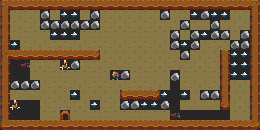
\includegraphics[scale=0.6, valign=c]{WarpedImages/boulderdashDefault.png}} \quad
  \subfloat[Warped Screen Observation for Boulderdash]{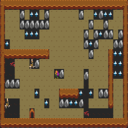
\includegraphics[scale=0.6, valign=c]{WarpedImages/boulderdashWarped.png}} \qquad
  \subfloat[Raw Screen Observation for Ikaruga]{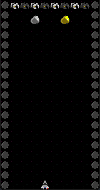
\includegraphics[scale=0.6, valign=c]{WarpedImages/ikarugaDefault.png}} \quad
  \subfloat[Warped Screen Observation for Ikaruga]{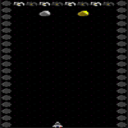
\includegraphics[scale=0.6, valign=c]{WarpedImages/ikarugaWarped.png}\label{fig:ikarugaWarped}}
  \caption{Comparison of Raw Screen Observations and Warped Screen Observations for two games}
  \label{fig:ScreenWarping}
\end{figure*}
Figure~\ref{fig:ScreenWarping} shows the effects of screen warping to a fixed size of 128x128 across a couple of games.
While it can be seen that some raw pixel information is lost during the process, elements of the games can still be seen and recognised as the down sampling effect isn't too dramatic.
Specifically as each game is made up of sprites and tiles and the warping doesn't reduce past a tile size, each tile can still be recognised.
Some games will have parts of the image up sampled as can be seen in figure~\ref{fig:ikarugaWarped}, where the x dimension has been up sampled.
\par
An advantage of applying some down sampling during the image warping process is the reduction of GPU VRAM needed during training.
As the images are physically smaller in size they take up less VRAM when stored on the GPU during each backpropagation step.
This value can then be tuned to allow for larger minibatches without overfilling the GPU VRAM.
This provides the benefit of allowing more parallel environments to run simultaneous, potentially speeding up training, and better GPU utilisation during training.

\subsection{Requiring Fixed Sized Input to the Model}
\label{ssec:fixedOutput}
As with the limitations for inputs to a neural network size, pointed out in section~\ref{ssec:fixedInput}, the output of a MLP needs to be a predetermined fixed size.
This is an issue as the number of accepted control inputs for games in the GVGAI framework vary from game to game.
\subsubsection{Action Representation in the GVGAI Framework}
Currently all of the games in the GVGAI framework use a combination of the following 6 actions:
\begin{multicols}{2}
\begin{itemize}
    \item Do Nothing
    \begin{itemize}
        \item ACTION\_NIL
    \end{itemize}
    \item Perform Action
    \begin{itemize}
        \item ACTION\_USE
    \end{itemize}
    \item Movement Actions
    \begin{itemize}
        \item ACTION\_LEFT
        \item ACTION\_RIGHT
        \item ACTION\_DOWN
        \item ACTION\_UP
    \end{itemize}
\end{itemize}
\end{multicols}
Games such as aliens (a space invaders style game) don't accept the actions ACTION\_UP and ACTION\_DOWN due to the lack of vertical movement in the game, therefore it only accepts 4 possible actions.
\par
Specifically in the GVGAI framework, these actions are represented as an integer number between 0-N exclusive where N is the total number of valid actions for that particular game.
Alongside the state observation at each time step, agents are given a list of available actions where the agent needs to return the list index of the action it wants to perform.
If an agent returns an invalid action ID then the agent is disqualified from that run, so there is a high penalty for trying to perform an invalid action.

\subsubsection{Creating a Fixed Output Layer Size}
As with the input layer of the neural network, the output layer has to be a fixed predetermined size.
To ensure the model can return actions for all games, the output of the model could be fixed to return an integer value between 0-6 exclusive.
\par
This would allow for an agent using this model to play approximately 40\% of the available games in the GVGAI framework, those that use all 6 actions.
This gives complications in the remaining 60\% of games that have a lower number of acceptable actions, as giving an invalid action at any time results in disqualification.
\subsubsection{Dropping Invalid Actions}
The proposed solution for dealing with games with a lower number of valid actions is for the agent to simply ignore invalid actions and send a ACTION\_NIL instead.
This can be achieved by comparing the action ID proposed with the length of the list of actions, dropping the action if its value is greater than or equal to the length of the list.
If an action is chosen to be dropped the agent can send the value of 0 as this corresponds to ACTION\_NIL for all games in the GVGAI framework.
\par
Doing nothing makes sense as the default state of the agent as it typically has the least impact on the state of the game.
Performing ACTION\_NIL is currently used as a way to penalise agents in the GVGAI game playing tracks that don't return an action within a given time frame without drastically going over time to result in disqualification.
This behaviour is also indicative of human play as humans don't have the reactions required to press a unique button every frame, so in human play most of the time no action is performed.
\subsubsection{Robustness of Dropping Invalid Actions}
While this method works for all current games in the GVGAI framework, it isn't robust to 2 changes to in future games due to a couple of assumptions made.
\par
The first assumption is that the maximum number of actions across all games is 6.
If a game was introduced with $>6$ actions the agent would never be able to use the actions corresponding to values~$>6$.
Although not using these actions wouldn't be grounds for disqualifying the agent, it would severely limit the agents ability to play those games as it doesn't have access to all the possible actions.
\par
The second assumption is that the action corresponding to the ID 0 is ACTION\_NIL.
Breaking this assumption could lead to unknown effects in many games depending on what the action that ID 0 mapped to.
During the learning phase it is theoretically possible that the agent could learn to not use these actions if they are detrimental to its progress.
\par
A final issue with this method is that the same ID values don't map to the same actions.
For example in Aliens action id 1 corresponds to ACTION\_USE, but in Camel Race this corresponds to ACTION\_LEFT.
This could be fixed by using the list of actions provided to the agent to translate between the model and the output, although this wasn't examined.

\subsection*{Combining Image Warping and Dropping Actions}
Through combining the methods in section~\ref{ssec:fixedInput} and section~\ref{ssec:fixedOutput} an agent with a single model can technically play all games and levels in the GVGAI framework.
This also allows for the neural network architecture to be designed separately to the agent and irespective of the games it can play.
The agent simply needs to know the input size the neural network requires to reshape the raw observation before feeding it through the neural network.

\subsection{Removing the Alpha Channel}
The raw state observation image that the agent receives is encoded as an 8-bit RGBA image.
Inclusion of an alpha channel in the raw state observation image doesn't make logical sense as typically a game doesn't have any transparency elements.
\par
After doing some analysis of all levels in the GVGAI framework it was determined that the alpha channel was redundant information.
For most of the games in the GVGAI framework the alpha channel isn't used, with the it simply being filled with 0s.
For the few games that do use the alpha channel the only values used are max (255) and zeros.
\par
The alpha channel is mostly used to show the locations of floors and walls in a maze-like games, something which is encoded in the RGB channels of the image too.
When a human player plays a game this information wouldn't be shown to them so inclusion of the alpha channel could also be seen as giving extra knowledge to the agent.
\par
The alpha channel was therefore removed from the raw state observation images by simply slicing it off before feeding it through the model.
This is done to reduce the dimensionality of the input data, allowing for few parameters needed to be learnt and quicker processing of the state observations.

\subsection{Scaling Rewards During Training}
While all the previous processing techniques are performed during both training and playing, this technique is only used during training to help normalise the rewards across all of the games.
Normalisation is a common technique used in machine learning to help speed up the training process.
The requirement for such a technique is motivated from how some games have higher or more frequent rewards than others.
\par
Mnih et al.~\cite{DeepAtari} tackled this by clipping all positive rewards to 1 and negative rewards to -1 when training on Atari games.
The authors mentioned that this `limits the scale of the error derivatives and makes it easier to use the same learning rate across multiple games', a useful feature for general video game playing.
They continued to suggest how this method could effect performance of the agent as `it cannot differentiate between rewards of different magnitude.'
\par
The method proposed here aims to tackle both the issue of higher total rewards, and more frequent rewards while retaining the ability to differentiate between different reward magnitudes.
To do this, all the rewards are scaled by a fraction of the maximum score achievable in that game.
\par
The scaled rewards are calculated by the following equation
\begin{equation} \label{eq:scalingReward}
    r\prime=r\times\frac{k}{m}
\end{equation}
Where $r\prime$ is the scaled reward, $r$ is the given reward, $k$ is the scaling factor, and $m$ is the maximum possible score in that level.
This also has the added benefit of showing how far off obtaining a perfect score an agent is during training by plotting the episode rewards, a common metric tracked in reinforcement learning.
\par
The use of the maximum score during training can be seen as a domain specific knowledge as it requires analysis of the game and levels used during training to figure out the maximum achievable score.
While this is true, at no point is the underlying model exploiting this domain specific knowledge with it being used to give equal priority to all games in the training set.

\subsection{Agent Structure}
These methods and the neural network model are integrated together in the form of an intelligent agent.
The overall agent can be classified as a purely reactive agent, without any internal memory.
At each time step the agent perceives the game via the raw screen image, which is processed to remove the alpha channel and warp to a fixed size before being processed by the underlying CNN which drives the agents decision making.
The action chosen by the CNN is checked to see if its a valid action and dropped if necessary, passing the final action decision onto the environment.
Figure~\ref{fig:agentStructure} shows this relationship diagrammatically.
\begin{figure}[h]
  \centering
  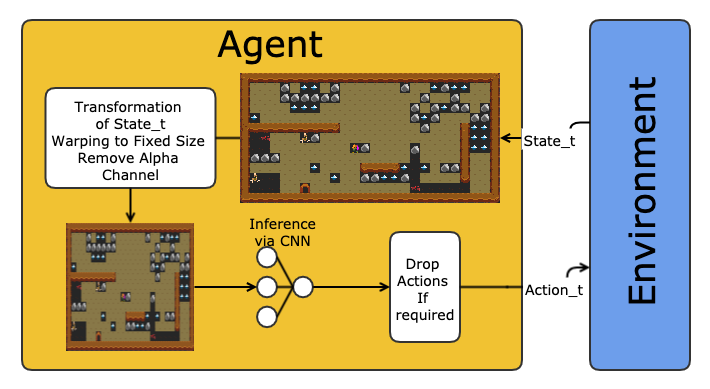
\includegraphics[width=0.7\linewidth]{figures/agentStructure.png}
  \caption{Agent Structure Diagram}
  \label{fig:agentStructure}
\end{figure}